\section{Problema 3 \textit{(Costruire un albero di costo minimo)}}

\subsection{Definizione dei sottoproblemi}

Nella risoluzione del problema, abbiamo focalizzato il nostro ragionamento sulle proprietà fondamentale che deve avere un albero per
essere accettabile, ovvero:
\begin{enumerate}
	\item Il costo complessivo dell'albero deve essere minimo.
	\item Ogni nodo interno deve avere esattamente due figli.
	\item L'albero ha  esattamente $n$ foglie.
\end{enumerate}

\begin{center}
	\textbf{$OPT[i, j]$ rappresenta l'albero di costo minimo contenente le foglie $\{C[j], C[j + 1], ..., C[j + i - 1]\}$ date in input, 
		$\forall i\ \in\ \{1, ..., n\} \land \forall j\ \in\ \{1, ..., n - i + 1\}$ dove $i$ indica la $i-esima$ riga e $j$ indica la $j-esima$ colonna della matrice $OPT$.}
\end{center}

\subsection{Struttura dati}

Abbiamo definito una matrice $OPT$ di dimensioni $n \times n$, dove ogni cella contiene 4 valori:

\begin{itemize}
	\item $OPT[i, j].val$: il costo minimo per costruire un albero con le foglie che vanno da $j$ a $j + i - 1$ (dove $i$ rappresenta le righe e $j$ le colonne).
	\item $OPT[i, j].max$: il valore massimo tra le foglie all'interno dell'intervallo $[j: j + i - 1]$.
	\item $OPT[i, j].sin$: le coppie di indici $i,\ j$ che all'interno di $OPT$ ci indicano quale cella guardare per ricostruire la struttura del sottoalbero sinistro.
	\item $OPT[i, j].des$: le coppie di indici $i,\ j$ che all'interno di $OPT$ ci indicano quale cella guardare per ricostruire la struttura del sottoalbero destro.
\end{itemize}

Tuttavia, è importante notare che utilizziamo solo la metà delle celle di $OPT$. In particolare,
ci limitiamo alla matrice triangolare superiore sinistra, poiché oltre questa 
zona andremmo oltre il numero di foglie salvate nell'array $C$, contenente i valori delle foglie dati in input.

\subsection{Combinazione dei sottoproblemi}

Nel processo di combinazione dei sottoproblemi, abbiamo tenuto presente che un albero ottimale deve essere strutturato in modo binario, cioè deve avere due 
sottoalberi per ogni nodo interno. Questa considerazione ci ha portato a distinguere le foglie in due gruppi: le "foglie destre", che appartengono al sottoalbero 
destro, e le "foglie sinistre", che appartengono al sottoalbero sinistro.

\subsubsection*{Casi base}

Durante l'analisi dei casi base, abbiamo individuato due situazioni:

\begin{itemize}
	\item {
		Il primo caso base riguarda la prima riga della matrice, dove ogni cella rappresenta una foglia singola. In questo caso, assegniamo il valore della foglia a $OPT[1, j].max$, 
		mentre poniamo il valore di $OPT[1, j].val = 0$ (poiché per la nostra definizione le foglie non hanno valore). $OPT[1, j].sin$ e $OPT[1, j].des$ non vengono inizializzate in quanto 
		non ci sono sottoalberi.
	}
	\item {
		Il secondo caso base si riferisce alla seconda riga della matrice, dove ogni cella rappresenta un albero con solo due foglie. Questo albero può essere combinato in un 
		unico modo, poiché le foglie devono essere ordinate secondo una visita simmetrica rispetto all'input. In questo caso, il valore di $OPT[2, j].val$ è il prodotto tra 
		gli $OPT[1, j].max$ e $OPT[1, j + 1].max$ i quali indicano le foglie, mentre $OPT[2, j].max$ rappresenta il massimo tra i due valori delle foglie. Inoltre, assegniamo gli indici delle foglie a $OPT[2, j].sin$ e $OPT[2, j].des$ 
		per poter trovare facilmente le loro posizioni nella matrice.
	}
\end{itemize}

\subsubsection*{Caso generico}

Avendo effettuato questa suddivisione tra sottoalbero destro e sottoalbero sinistro, ci siamo resi conto che la chiave per trovare il valore dell'albero 
ottimale consiste nel provare tutte le possibili suddivisioni fra foglie destre e sinistre e trovare quella con il costo complessivo minimo. Questo si riduce a 
cercare un indice $k$ nell'intervallo $[1 : i - 1]$ tale che il nodo risultante dalla combinazione del sottoalbero sinistro contenente le foglie da $j$ a $j + k$ e del 
sottoalbero destro contenente le foglie da $j + k +1$ a $j + i - 1$ sia il più piccolo possibile in termini di costo.

\newpage
\subsubsection*{Numero dei sottoproblemi}

Per come sono stati definiti i sottoproblemi, ciascun sottoproblema corrisponde ad una cella della matrice triangolare superiore sinistra. A tal proposito 
il numero di sottoproblemi è $\frac{n^2}{2} = O(n^2)$. 

\subsubsection*{Goal}

Il valore dell'albero minimo che stiamo cercando si trova all'interno della cella $OPT[n,1].val$.\\
Questa cella contiene il valore dell'albero minimo che include tutte le foglie che vanno da 
$C[1]$ a $C[n]$ (essendo $i = 1$ e $j = n$). 
Poiché questo albero contiene tutte le foglie, è l'albero di costo minimo che stiamo cercando.


\subsection{Formula di Bellman}

\subsubsection*{Caso base, $i = 1$}

\begin{align*}
	OPT[i, j]	
	\begin{cases}
		.val = 0\\                                                                                          
		.max = C[j]\\
		.sin = NULL\\
		.des = NULL\\
	\end{cases}                                                                                            
\end{align*}


\subsubsection*{Caso base, $i = 2$}

\begin{align*}
	OPT[i, j]	
	\begin{cases}
		.val = OPT[i - 1, j].max \times OPT[i - 1, j + 1].max\\                                                                                          
		.max = \max\{OPT[i - 1, j].max, OPT[i - 1, j + 1].max\}\\
		.sin = (i - 1, j)\\
		.des = (i - 1, j + 1)\\
	\end{cases}                                                                                            
\end{align*}

\subsubsection*{Caso generico}

$$
OPT[i, j].val = \min_{k = 1,\ \dots,\ i - 1}\{(OPT[k, j].max \times OPT[i - k, j + k].max) + OPT[k, j].val + OPT[i - k, j + k].val\}
$$

Dopo aver trovato il $k$ che minimizza la formula sopra, calcoliamo i restanti 3 campi di $OPT[i, j]$

\begin{align*}
	OPT[i, j]	
	\begin{cases}                                                                                          
		.max = \max\{(OPT[k, j].max, OPT[i - k, j + k].max)\}\\
		.sin = (k, j)\\
		.des = (i - k, j + k)\\
	\end{cases}                                                                                            
\end{align*}



\subsubsection*{Esempio}

Supponiamo di avere in input il seguente vettore $C = [4, 2, 7]$ con 3 foglie.

Ogni cella della matrice contiene 4 valori, dunque possiamo codificare questi 4 valori come 
il seguente array: $[.val, .max, .sin, .des]$.

\[
	\begin{bmatrix}
		[0, 4, -, -]           & [0, 2, -, -]            & [0, 7, -, -] \\
		[8, 4, (1, 1), (1, 2)] & [7, 14, (1, 2), (1, 3)] & [-, -, -, -] \\
		[?, ?, ?, ?]           & [-, -, -, -]            & [-, -, -, -] \\
	\end{bmatrix}
\]

Per riempire la cella $OPT[3, 1]$, che contiene il valore dell'albero minimo, 
dobbiamo determinare la combinazione ottimale delle foglie che produce l'albero di costo minimo. 
Quindi, dobbiamo trovare l'indice $k$ compreso tra $1$ e $i - 1$. Considerando la cella $(3, 1)$, 
dove $i = 3$, i possibili valori per $k$ sono $1$ e $2$.


\begin{center}
	\begin{enumerate*}[label={}]
	\item {
		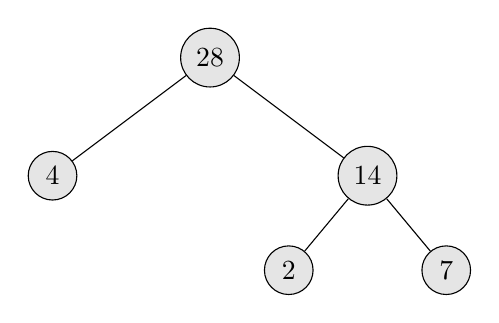
\begin{tikzpicture}[
				level/.style={sibling distance=40mm/#1},
				every node/.style={circle, draw, fill=black!10},
				level 1/.style={level distance=15mm},
				level 2/.style={level distance=12mm},
				level 3/.style={level distance=10mm}
			]
			\node {28}
			child {node {4}}
			child {node {14}
				child {node {2}}
				child {node {7}}
			};
		\end{tikzpicture}
	}
	\newline
	\item{
	      Con $k = 1$ dobbiamo combinare i valori contenuti in $OPT[1,1]$ e $OPT[2,2]$, portando così il costo dell'allbero a 42
	}
\end{enumerate*}
\end{center}


\begin{center}	
\begin{enumerate*}[label={}]
	\item {
		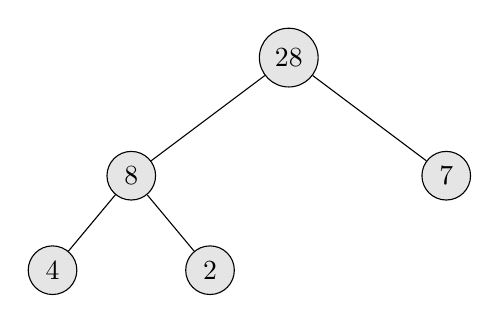
\begin{tikzpicture}[
				level/.style={sibling distance=40mm/#1},
				every node/.style={circle, draw, fill=black!10},
				level 1/.style={level distance=15mm},
				level 2/.style={level distance=12mm},
				level 3/.style={level distance=10mm}
			]
			\node {28}
			child {node {8}
				child {node {4}}
				child {node {2}}
			}
			child {node {7}};
		\end{tikzpicture}
	}
	\newline
	\item{
		Con $k = 2$ dobbiamo combinare i valori contenuti in $OPT[2,1]$ e $OPT[1,3]$, portando così il costo dell'allbero a 36
	}
\end{enumerate*}
\end{center}


\[
	\begin{bmatrix}
		[0, 4, -, -]            & [0, 2, -, -]            & [0, 7, -, -] \\
		[8, 4, (1, 1), (1, 2)]  & [7, 14, (1, 2), (1, 3)] & [-, -, -, -] \\
		[36, 7, (2, 1), (1, 3)] & [-, -, -, -]            & [-, -, -, -] \\
	\end{bmatrix}
\]


\subsection{Pseudocodice}


\begin{algorithm}
	\caption{Algoritmo\_Albero}
	\begin{algorithmic}[1]
		\Function{compute\_opt}{C[1: n]}
		\State \textbf{Matrix} $OPT[n, n]$ 
		\State \Comment{Caso base, $i = 1$}
		\For{$j = 1$ \textbf{to} $n$}
		\State $OPT[1, j].val = 0$
		\State $OPT[1, j].max = C[j]$
		\State $OPT[1, j].sin = NULL$
		\State $OPT[1, j].des = NULL$
		\EndFor

		\State \Comment{Caso base, $i = 2$}

		\If{$n >= 2$}
		\For{$j = 1$ \textbf{to} $n$}
		\State $OPT[2, j].val = OPT[i - 1, j].max \times OPT[i - 1, j + 1].max$
		\State $OPT[2, j].max = \max\{OPT[i - 1, j].max, OPT[i - 1, j + 1].max\}$
		\State $OPT[2, j].sin = (i - 1, j)$
		\State $OPT[2, j].des = (i - 1, j + 1)$
		\EndFor
		\EndIf
		\State \Comment{Fine casi base}

		\State \Comment{Casi Generici}
		\If{$n >= 3$}
		\For{$i = 1$ \textbf{to} $n$}
		\For{$j = 1$ \textbf{to} $n - i + 1$}
		\State $OPT[i, j].val = \min_{k = 1,\ \dots,\ i - 1}\{(OPT[k, j].max \times OPT[i - k, j + k].max) + OPT[k, j].val + OPT[i - k, j + k].val\}$
		\State Salviamo il $k$ che minimizza $OPT[i, j].val$
		\State $OPT[i, j].max = \max\{(OPT[k, j].max, OPT[i - k, j + k].max)\}$
		\State $OPT[i, j].sin = (k, j)$
		\State $OPT[i, j].des = (i - k, j + k)$
		\EndFor
		\EndFor
		\EndIf
		
		\Return $OPT[n, 1].val$
		\EndFunction
	\end{algorithmic}
\end{algorithm}

\subsubsection*{Analisi della complessità}

\begin{itemize}
	\item{
		Il tempo di esecuzione dell'algoritmo è una diretta conseguenza del numero dei sottoproblemi. Infatti avendo $O(n^2)$ sottoproblemi,
		ciascuno risolvibile in tempo $O(k)$, segue che l'algoritmo trova la soluzione ottima in tempo $O(n^2 \times k)$, dove $k = O(n)$. 
		In conlusione il tempo di esecuzione è $O(n^3)$.\\
		Siamo consapevoli che la complessità temporale di questo algoritmo non sia ottimale.
	}
	\item{
		Per quanto riguarda lo spazio utilizzato, usando la tecnica tabulation, in memoria salviamo una matrice $n \times n$ dove ciascuna cella contiene 4 valori.
		Di conseguenza, l'algoritmo calcola la soluzione ottima in spazio $4n^2 = O(n^2)$.
	}
\end{itemize}

\subsection{Ricostruzione dell'albero}

Per quanto concerne la ricostruzione dell'albero, a partire dalla matrice $OPT$, in tempo lineare nel numero di nodi dell'albero possiamo ricostruire l'albero nel seguente modo:

\begin{itemize}
	\item Partiamo dalla cella $OPT[n, 1]$, che contiene la radice dell'albero, in quanto contiene la somma dei valori dei nodi interni dell'albero.
	\item {
		Il valore di ciascun nodo lo ricaviamo guardando le coppie degli indici $.sin$ e $.des$.\\
		Definiamo $sin_{i,j} = OPT[i, j].sin$ e $des_{i,j} = OPT[i, j].des$.\\
		Dunque, il valore della radice è:\\
		$root = OPT[n, 1].val - (OPT[sin_{n,1}].val + OPT[des_{n, 1}].val)$
		}
	\item {
		In generale, per un nodo $x_{i,j}$, $val(x_{i,j}) = OPT[i, j].val - (OPT[sin_{i,j}].val + OPT[des_{i,j}.val])$
	}
\end{itemize}

Per comodità, assumiamo $sin = (sin_{0},\ sin_{1})$ e $des = (des_{0},\ des_{1})$, quindi
$$
OPT[sin] = OPT[sin_{0},\ sin_{1}]
$$
$$
OPT[des] = OPT[des_{0},\ des_{1}]
$$ 

\begin{algorithm}
	\caption{RicostruzioneAlbero(OPT)}
	\begin{algorithmic}[1]
		\Function{RicostruzioneAlbero}{OPT}
		\State $T \gets$ albero vuoto
		\State $sin \gets OPT[n, 1].sin$
		\State $des \gets OPT[n, 1].des$
		\\
		\If{$sin = NULL$ \textbf{and} $des = NULL$} \Comment{foglia}
		\State $T.root \gets OPT[i, j].max$
		\State \Return $T$
		\EndIf
		\\
		\State $T.root \gets OPT[n, 1].val - (OPT[sin].val + OPT[des].val)$
		\State \Call{RicostruzioneAlberoRicorsivo}{OPT, T, sin[0], sin[1], root}
		\State \Call{RicostruzioneAlberoRicorsivo}{OPT, T, des[0], des[1], root}
		\\
		\State \Return $T$
	\EndFunction
\\
\\
	\Function{RicostruzioneAlberoRicorsivo}{OPT, T, i, j, parent}
	\State $sin \gets OPT[i, j].sin$
	\State $des \gets OPT[i, j].des$
	\\
	\If{$sin = NULL$ \textbf{and} $des = NULL$} \Comment{foglia}
	\State $val \gets OPT[i, j].max$
	\State \Return
	\EndIf
	\\
	\State $v.val \gets OPT[i, j].val - (OPT[sin].val + OPT[des].val)$
	\State rendi $v$ figlio di $parent$ in $T$
	\\
	\State \Call{RicostruzioneAlberoRicorsivo}{OPT, T, sin[0], sin[1], v}
	\State \Call{RicostruzioneAlberoRicorsivo}{OPT, T, des[0], des[1], v}
	\EndFunction

\end{algorithmic}
\end{algorithm}